\section{Modularity}
\label{sec:modularity}

\fxfatal{Relates to my work how?}

Since the framework developed in the course of this thesis is required to be highly modular, we first need to define the term \textit{Modularity}, find out how it relates to software engineering and choose a tool for supporting modularity on the Java platform.

Modularity is a frequently used term in Software Engineering. To understand the fundamental concept of it, take a look at the following definitions:

\begin{quote}
Large software systems are inherently more complex to develop and maintain than smaller systems. Modularity involves breaking a large system into separate physical entities that ultimately makes the system easier to understand. By understanding the behaviors contained within a module and the dependencies that exist between modules, it’s easier to identify and assess the ramification of change.

\hfill \textbf{Java Application Architecture}

\hfill \citeauthor{Knoernschild:2012} \cite{Knoernschild:2012}
\end{quote}

\begin{quote}
The term modularity is widely used in studies of technological and organizational systems. Product systems are deemed “modular”, for example, when they can be decomposed into a number of components that may be mixed and matched in a variety of configurations. The components are able to connect, interact, or exchange resources (such as energy or data) in some way, by adhering to a standardized interface. Unlike a tightly integrated product whereby each component is designed to work specifically (and often exclusively) with other particular components in a tightly coupled system, modular products are systems of components that are “loosely coupled".

\hfill \textbf{Modularity}

\hfill \citeauthor{Wikipedia:Modularity:2012} \cite{Wikipedia:Modularity:2012}
\end{quote}

Basically, modularity is based on modules, their requirements and behaviour. To fully understand the meaning of modularity we need to focus on the \textit{module} itself:

\subsection{Module definition}
\label{sec:module}

According to \citeauthor{Knoernschild:2012}, a software module is defined as follows:

\begin{quote}
A software module is a deployable, manageable, natively reusable, composable, stateless unit of software that provides a concise interface to consumers. 

\hfill \textbf{Java Application Architecture}

\hfill \citeauthor{Knoernschild:2012} \cite{Knoernschild:2012}
\end{quote}

\begin{figure}[H]
\centering
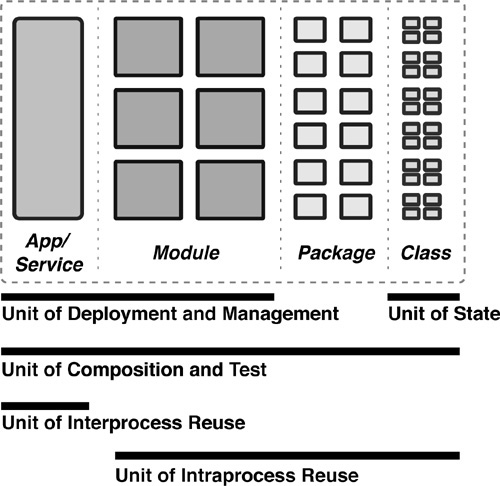
\includegraphics[width=0.7\textwidth]{module.jpeg}
\caption{Module definition diagram}
\label{fig:module}
\end{figure}

Figure \ref{fig:module} illustrates this defnition and all the individual aspects of a module will be explained in the following paragraphs \cite{Knoernschild:2012}:

\newpage
\subsubsection{Deployability}
Modules are deployable units and represent something more physical and coarse-grained than classes or packages. Examples of deployable units of software include EAR, WAR, and JAR files.

\subsubsection{Manageability}
Modules are manageable units and can be installed, uninstalled and refreshed. Modules allow for a better build efficiency and independent and therefore parallel development process.

\subsubsection{Testability}
Modules are testable units and can be tested independently and in isolation, very similar to classes in \gls{TDD}.

\subsubsection{Native Reusability}
Modules are units of intraprocess reuse. Unlike applications or services, modules are not a distributed computing technology. Instead, modularity is a way to organize units of deployment in a way that they can be reused across applications, but a module is always invoked natively.

\subsubsection{Composability}
Modules are composable units and can be composed of other modules. Usually coarse-grained modules are composed of finer-grained modules.

\subsubsection{Statelessness}
Modules are stateless and exist only as a single instance per version. We don’t instantiate software modules, although we do instantiate instances of the classes within software modules, and these classes may maintain state. However, the module itself does not.

\subsection{OSGi}
\gls{OSGi} is the most widely used and highly developed module system and service platform for the Java environment. This chapter aims to show why \gls{OSGi} is the best choice for building highly modular Java-based software systems.

The \gls{OSGi} technology is a set of specifications that define a dynamic component system for Java. These specifications enable a development model where applications are dynamically composed of many different reusable components. The \gls{OSGi} specifications enable modules to hide their implementations from other modules while communicating through services, which are objects that are specifically shared between modules. This surprisingly simple model has far reaching effects for almost any aspect of the software development process \cite{OSGi}. In OSGi parlance, a module is known as a bundle. OSGi provides a framework for managing bundles that are packaged as regular Java JAR files with an accompanying manifest. The manifest contains important metadata that describes the bundles and its dependencies to the OSGi framework \cite{Knoernschild:2012}. Figure \ref{fig:layering-osgi} shows the layered model architecture of the \gls{OSGi} service platform.

\begin{figure}[H]
\centering
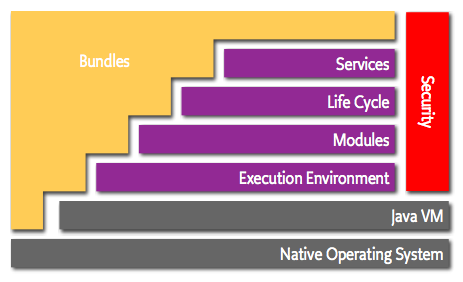
\includegraphics[width=0.73\textwidth]{layering-osgi.png}
\caption{\gls{OSGi} layered model \cite{OSGi}}
\label{fig:layering-osgi}
\end{figure}

\newpage
In summary, the \gls{OSGi} service platform offers the following features \cite{Knoernschild:2012}:

\begin{itemize}
	\item \textbf{Modularity}: \\
	Enables and enforces a modular approach to architecture on the Java platform.
	\item \textbf{Versioning}: \\
	Supports multiple versions of the same software module deployed within the same Java Virtual Machine (JVM) instance.
	\item \textbf{Hot deployments}: \\
	Permits modules to be deployed and updated within a running system without restarting the application or the JVM.
	\item \textbf{Encapsulation}: \\
	Allows modules to hide their implementation details from consuming modules.
	\item \textbf{Service orientation}: \\
	Encourages service-oriented design principles in a more granular level within the JVM. To accomplish this, OSGi uses $\mu$Services.
	\item \textbf{Dependency management}: \\
	Requires explicit declaration of dependencies between modules.
\end{itemize}

\newpage
\subsubsection{Specification versions}
The \gls{OSGi} specification is under constant development and the most current version is \textit{R5}, published in June 2012.

\begin{table}[H]
\centering
\begin{tabular*}{\textwidth}{ l l l }
	\toprule
	Name & Version & Date \\
	\midrule
	OSGi Release 1 & R1 & May 2000 \\
	OSGi Release 2 & R2 & Octover 2001 \\
	OSGi Release 3 & R3 & March 2003 \\
	OSGi Release 4 & R4 & October 2005 / September 2006 \\
	OSGi Release 4.1 & R4.1 & May 2007 \\
	OSGi Release 4.2 & R4.2 & September 2009 \\
	OSGi Release 4.3 & R4.3 & April 2011 \\
	OSGi Release 5 & R5 & June 2012 \\
	\bottomrule
\end{tabular*}
\caption{OSGi specification versions}
\label{tbl:osgi-versions}
\end{table}

Table \ref{tbl:osgi-versions} shows that OSGi is a proven, reliable platform specification, that is under continuous development for many years.

\subsubsection{Implementations}
\gls{OSGi} is the foundation for many different Application Servers and IDEs. Some of the most widely used open source implementations of the \gls{OSGi} specification are listed here: 

\begin{itemize}
	\item \textbf{Eclipse Equinox} \\
		\url{http://eclipse.org/equinox/} \\
		Equinox is the core of the plug-in runtime for the Eclipse IDE.
	\item \textbf{Apache Felix} \\
		\url{http://felix.apache.org/} \\
		Apache Felix is the open source \gls{OSGi} implementation powered by the \gls{ASF} and is the basis of several other Apache projects like Apache Aries and Apache Karaf.
	\item \textbf{Knopflerfish} \\
		\url{http://www.knopflerfish.org/} \\
		Knopflerfish is the spin-off from one of the \gls{OSGi} alliance founding members and was open-sourced in 2003.
\end{itemize}

Banshie uses Apache Felix for bundle testing purposes but aims to be \gls{OSGi} compliant and implementation independence. Apache Felix was chosen for its easy configuration and small memory footprint.

\subsection{Summary}
\fxfatal{Outro}